\documentclass[fleqn]{article}
\usepackage{graphicx}
\usepackage{subfig}
\usepackage{hyperref}

\begin{document}

\title{CMSC724 Project Progress Report\\\textit{A Metadata Platform of the Experimental Datasets for Computer Science}}
\author{Jinfeng Rao, Xing Niu}
\maketitle

This project consists of two main phrases: metadata extraction and metadata platform construction. At this stage, we are working on the first step and the objective is extracting fundamental metadata (e.g. data source, keywords, descriptions and usage in literatures) of datasets from computer science literatures.

We will talk about our current work on data preparing and modeling. The future work will also be introduced.

\begin{figure}[htbp]
\centering
\subfloat[Paper 1: Probability Estimates for Multi-class Classification by Pairwise Coupling]{
\label{fig:e1}
\fbox{
  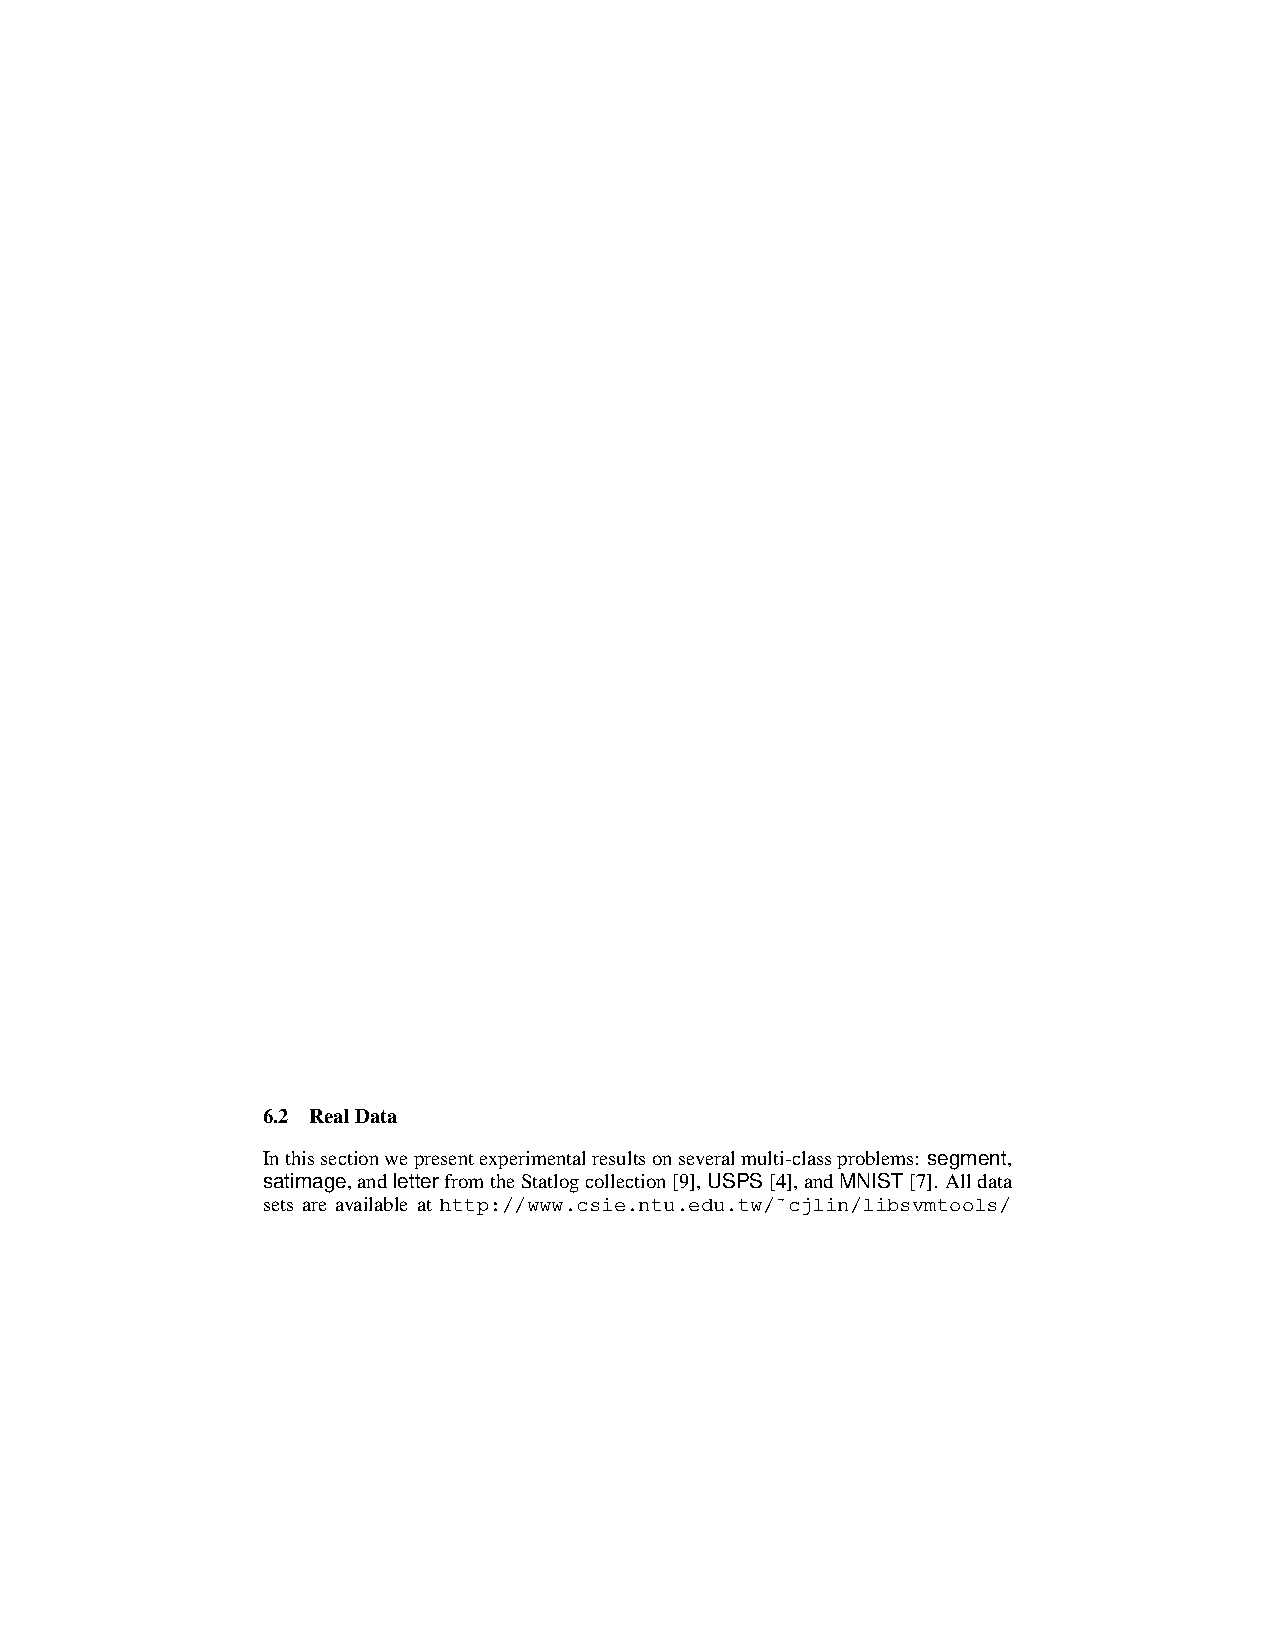
\includegraphics[width=0.9\textwidth]{examples/e1}
  }
}\\
\subfloat[Paper 2: Training Invariant Support Vector Machines]{
\label{fig:e2}
\fbox{
  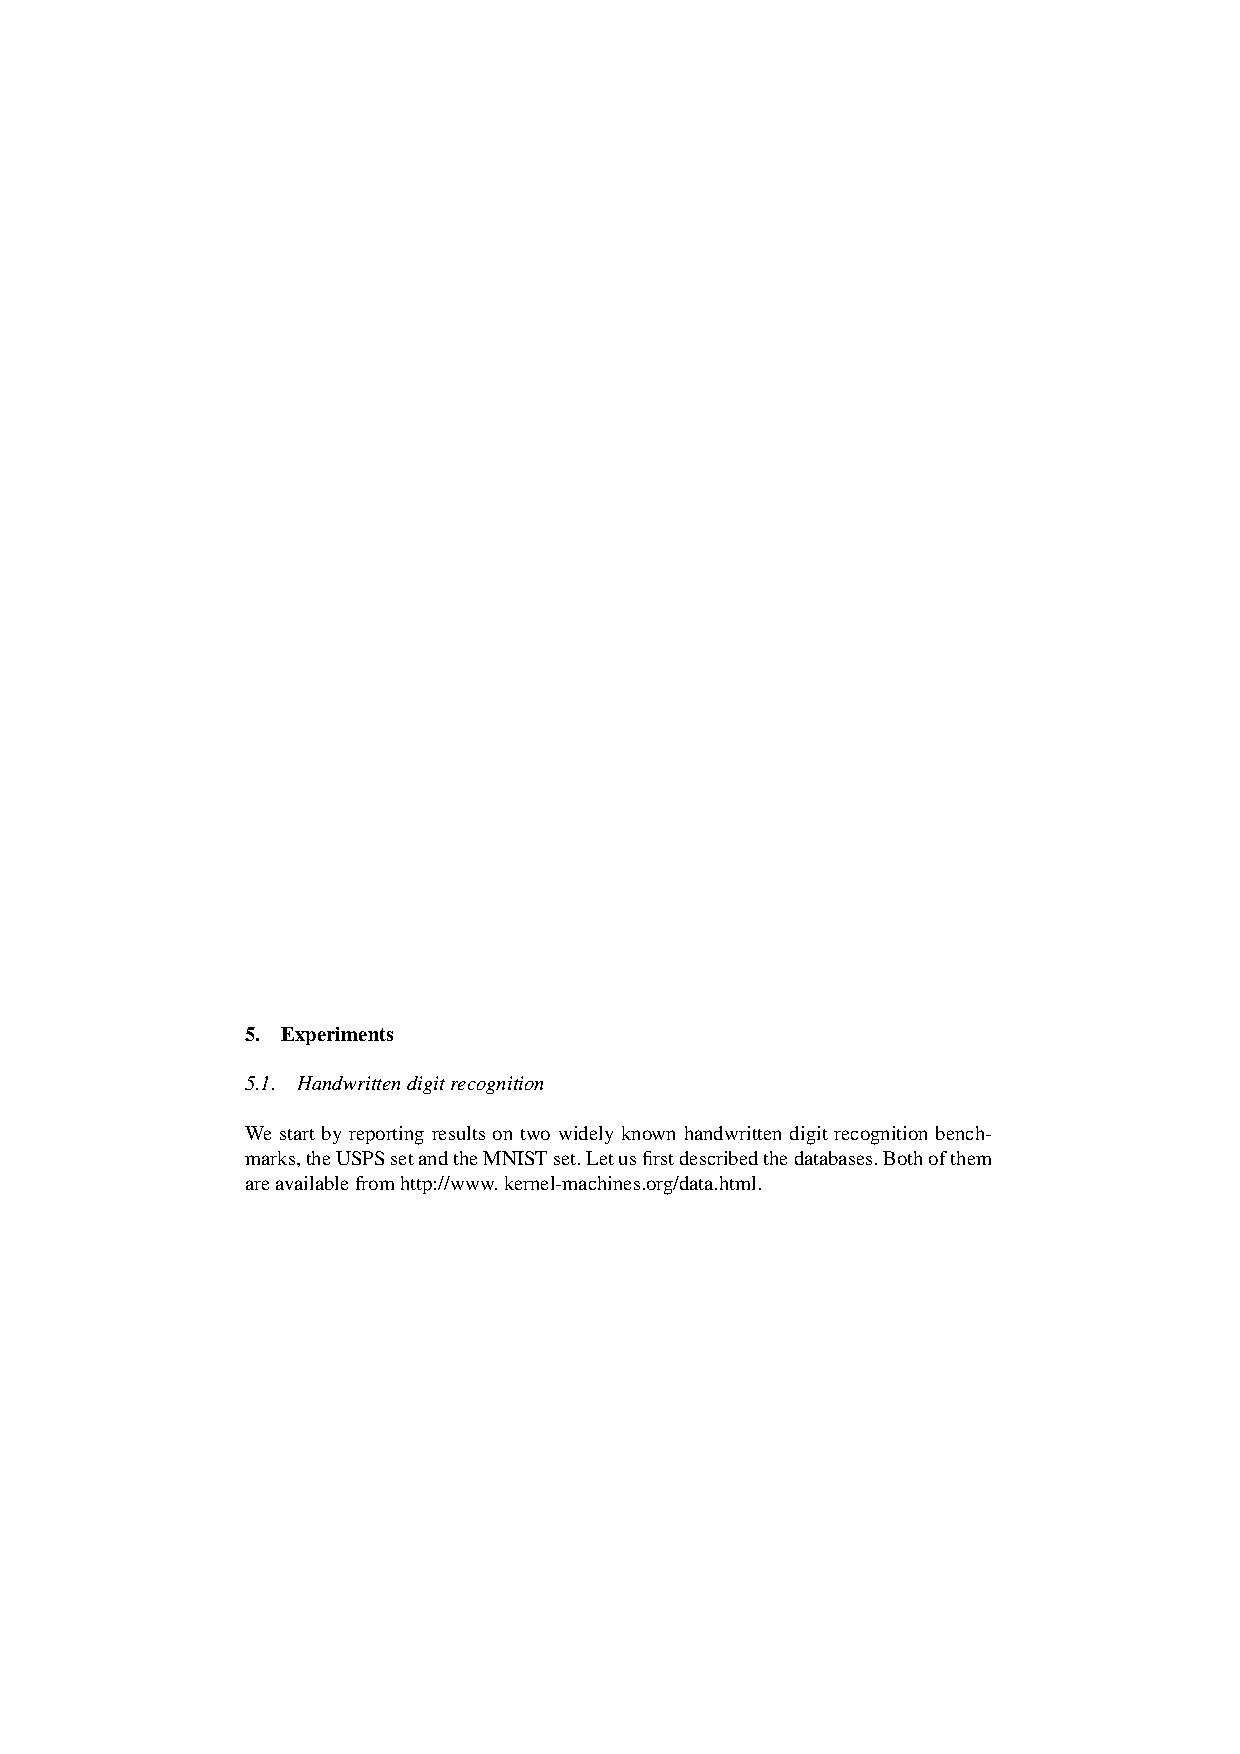
\includegraphics[width=0.9\textwidth]{examples/e2}
  }
}\\
\subfloat[Paper 3: A Fast Learning Algorithm for Deep Belief Nets]{
\label{fig:e3}
\fbox{
  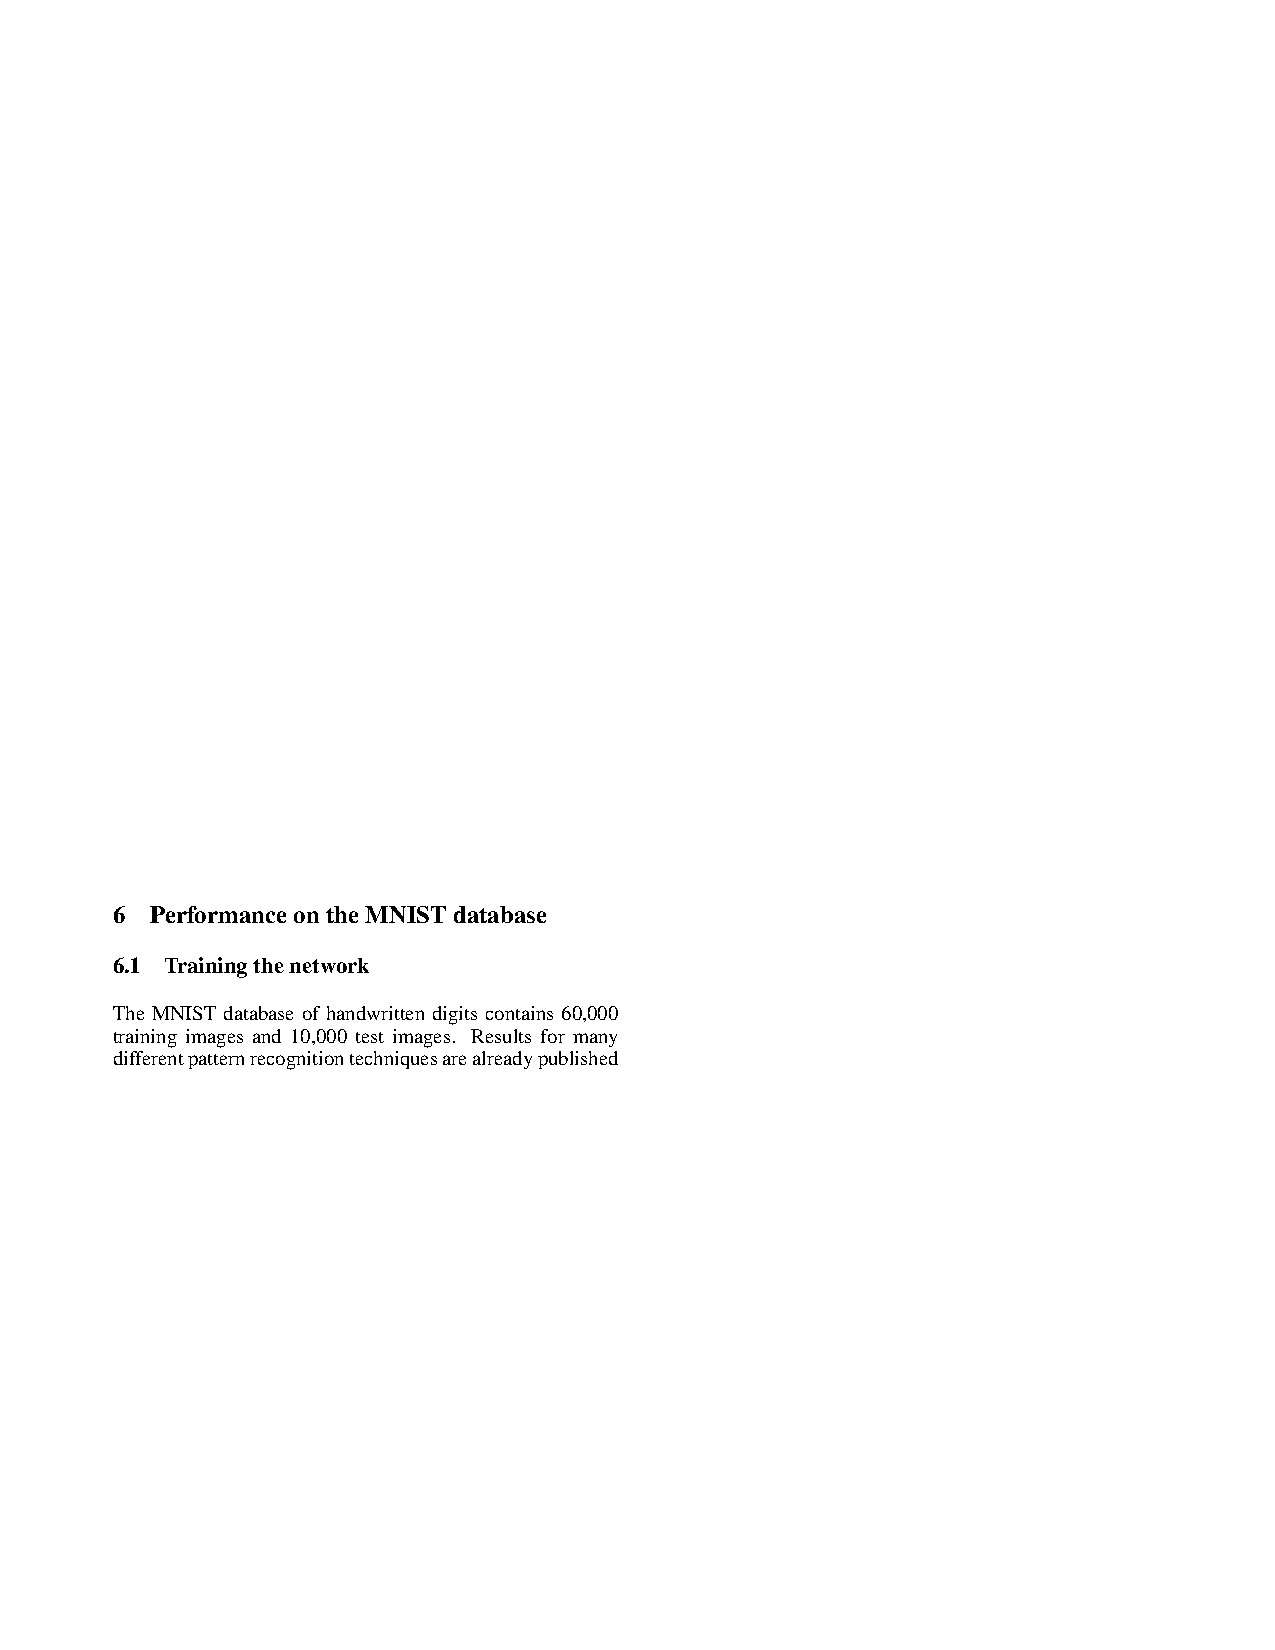
\includegraphics[width=0.9\textwidth]{examples/e3}
  }
}\\
\subfloat[Paper 4: Unsupervised Learning of Invariant Feature Hierarchies with Applications to Object Recognition]{
\label{fig:e4}
\fbox{
  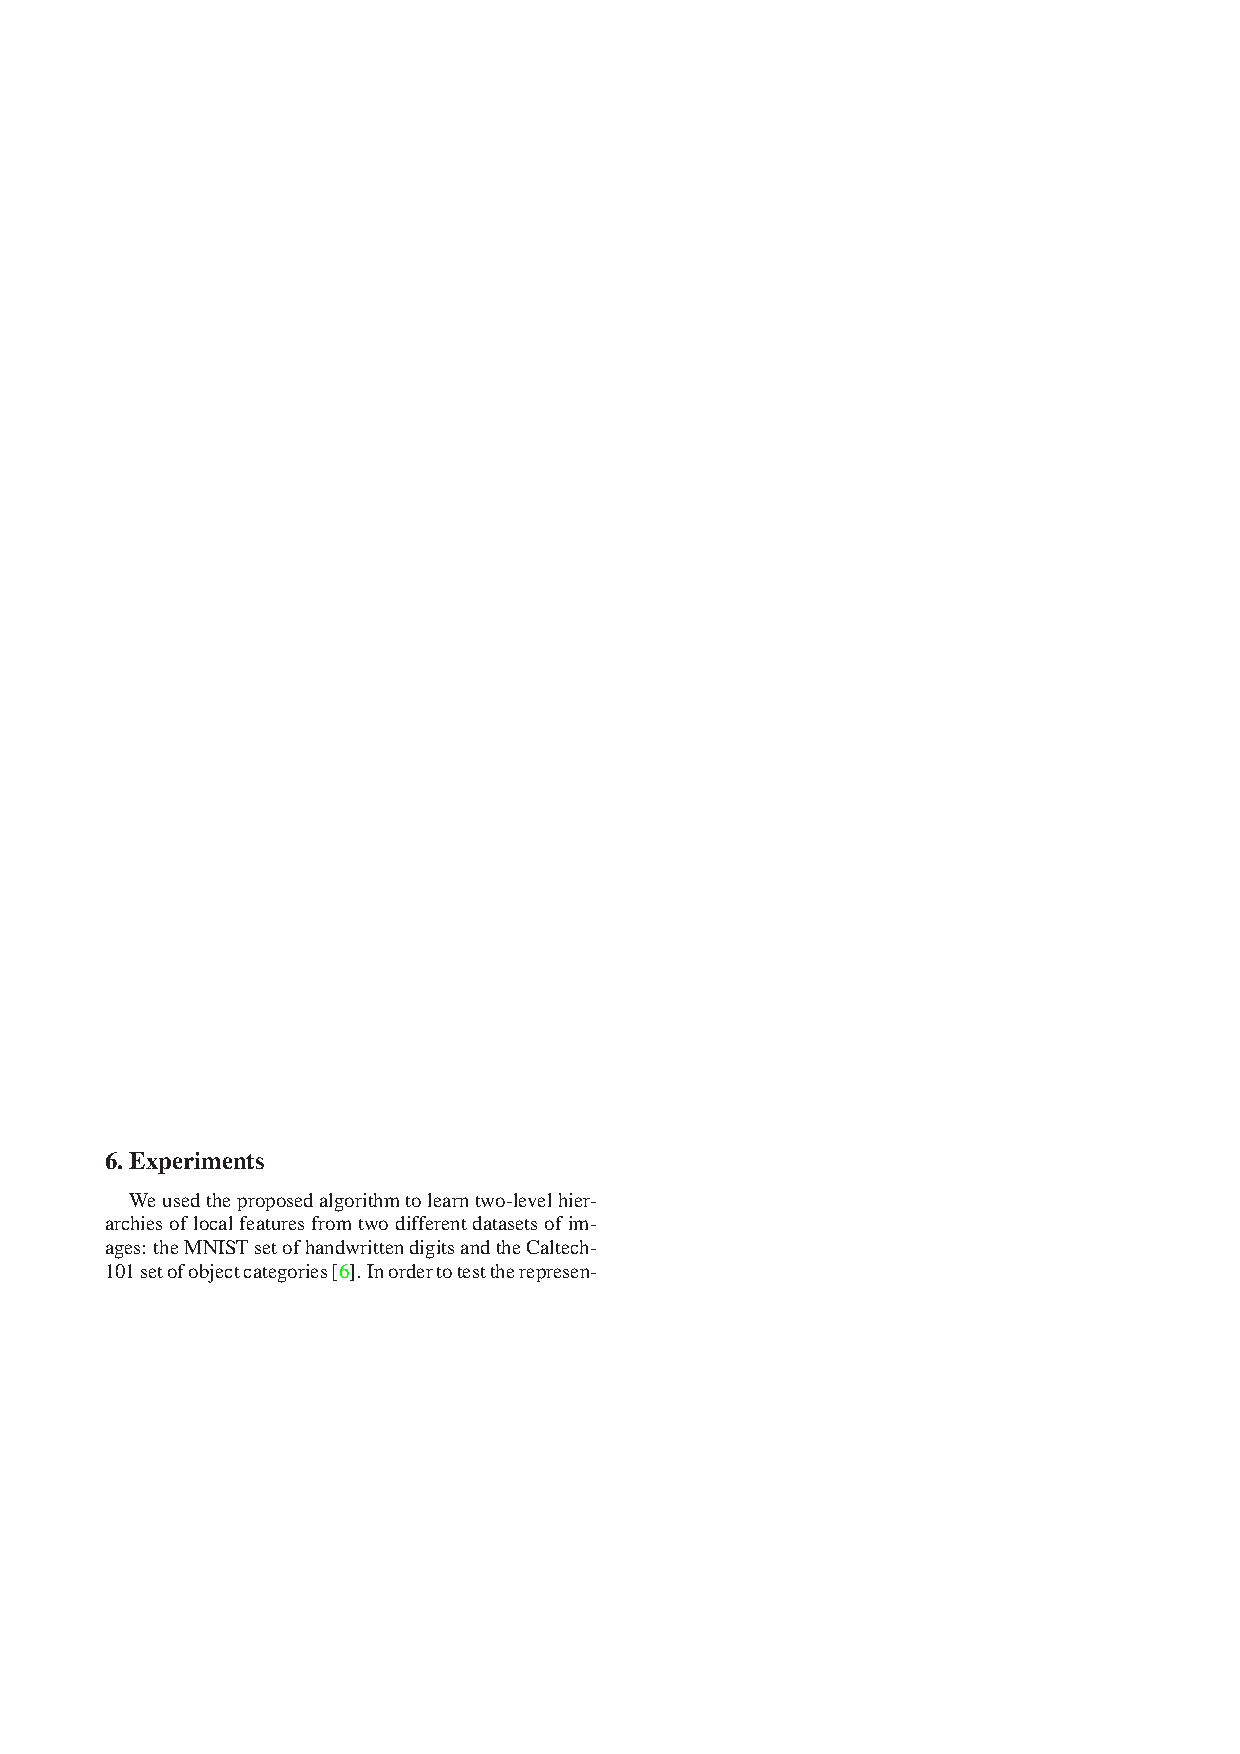
\includegraphics[width=0.9\textwidth]{examples/e4}
  }
}
\caption{Different descriptions for MNIST.}
\label{fig:e}
\end{figure}

\section{Data Preparing}
\subsection{Literature Repository}
Most research literatures are copyrighted, and we are not allowed to download too many articles from subscribed database (e.g. IEEE Xplore, ACM Digital Library) in a short period of time via our university's library. We try an alternative solution that use a Web crawler to dump articles from free academic databases such as arXiv.

The arXiv is a repository of electronic preprints of non-peer-reviewed scientific papers. Instead, a collection of moderators review the submissions. The quality of these papers varies, so we use them for testing our preliminary models since they can be easily accessed.

We plan to dump more standard research papers from academic search engines such as Google Scholar and CiteSeerX.

\subsection{Data Preprocessing}
Since all research papers in our project are assumed to be in the pdf format, a number of preprocessing techniques are employed for generating training data.

We use a PDF parser to convert pdf files to plain texts. Generally, structure and formating information (e.g. outlines and boldface) will be lost during the conversion. We have to group texts according to their original layout.

Grouping text chunks are used to locate specific and interesting content such as the title and keywords for a research paper. Another important text group is the section of experiment. Authors may name this section in different ways, such as ``results", ``evaluation" and ``setup".

\section{Modeling}
The reference sentences for dataset names usually follow some patterns such as ``the XXX dataset", ``XXX is a set of". Meanwhile, they are usually followed by a detailed description such as ``this dataset contains YYY" or ``it contains YYY". The challenge for us is automatically identifying such patterns. 

Since this is not a standard research topic, we have no labeled data/benchmarks at hand that have already identified dataset names in some papers. A related topic, named entity recognition, at least equipped with dictionaries. This condition restricts us to employ an unsupervised or semi-supervised learning method.

A reasonable solution is manually labeling a small quantity of data and using a bootstrapping framework to generate labels and rules incrementally.

\begin{description}
\item[Heuristic Rules.] Suppose we have known some dataset names (by manual labeling or by automatic candidate generation), the reference sentences as well as descriptions could be easily located. For example, as illustrated in Figure \ref{fig:e}, all sentences mention ``MNIST" can be seen as an instance of patterns.

\begin{figure}[hb]
\centering
\fbox{
   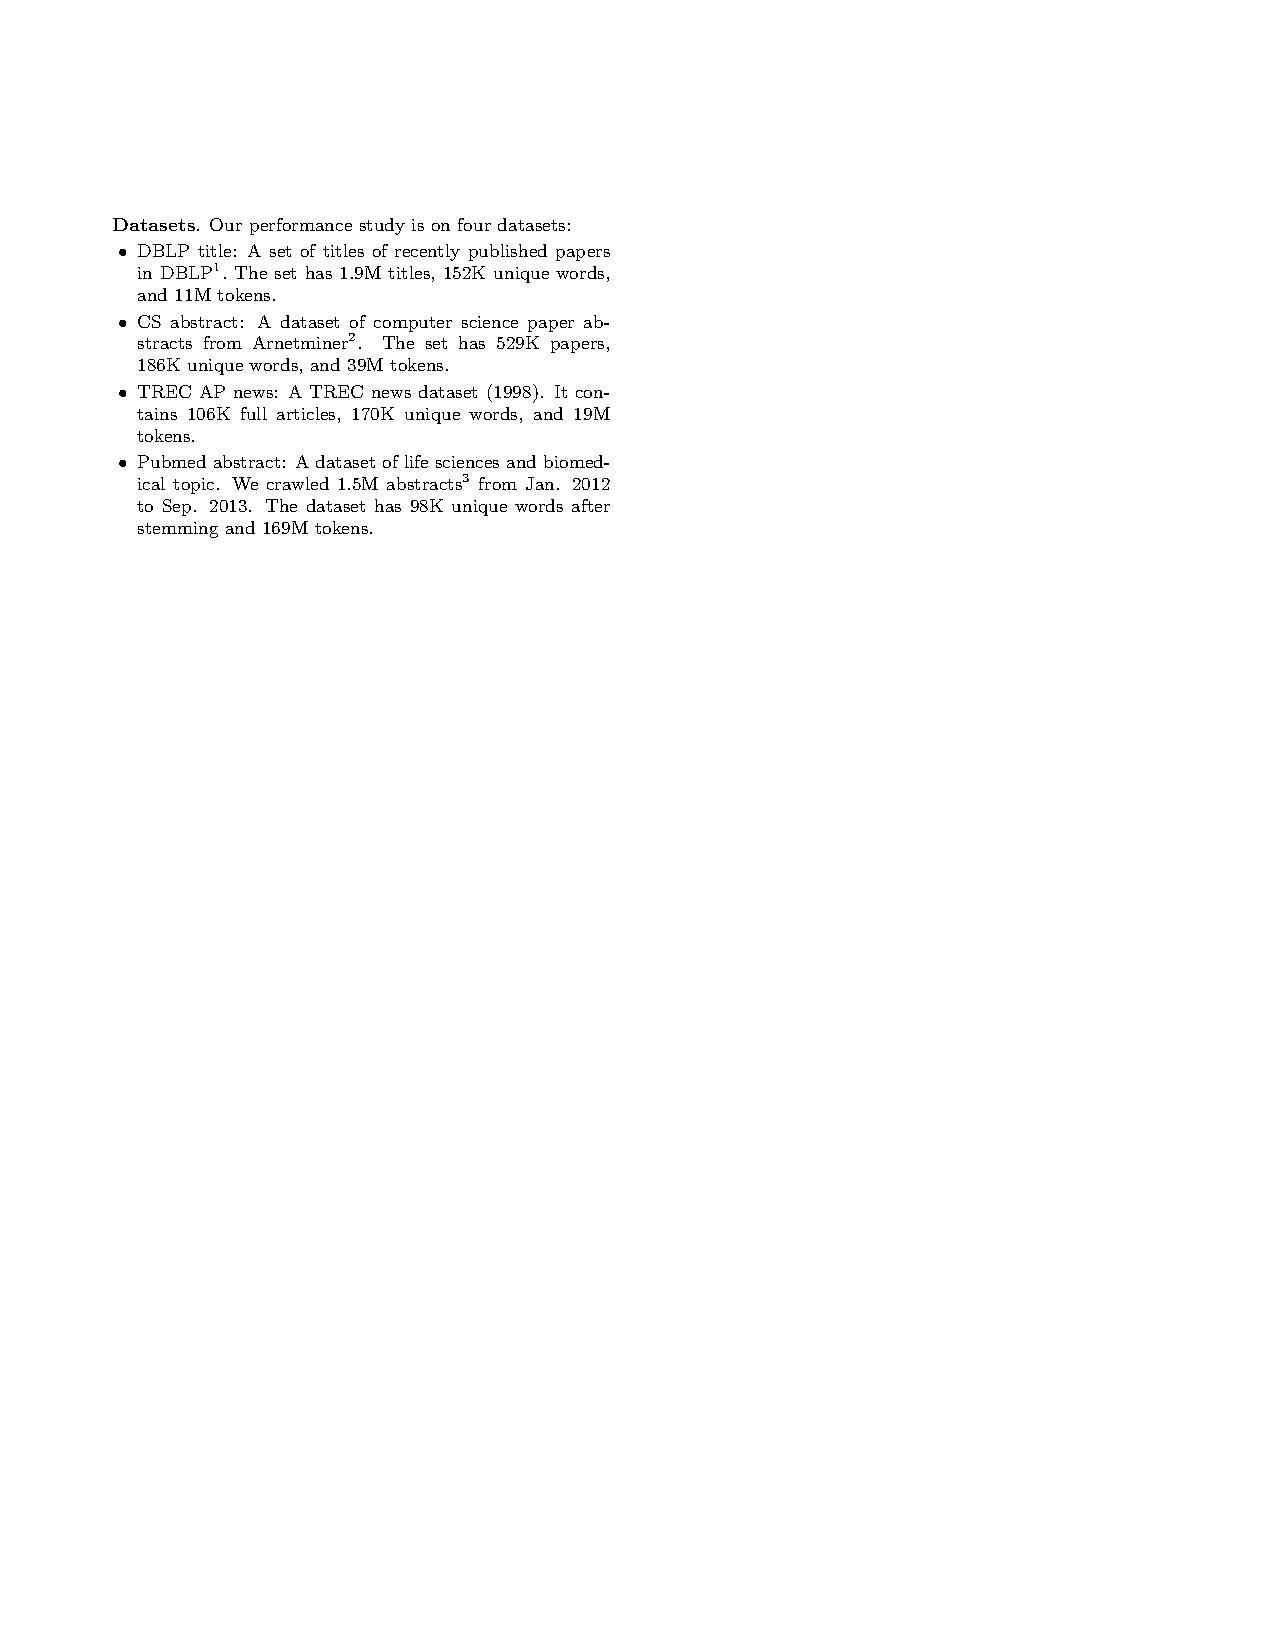
\includegraphics[width=0.8\linewidth]{examples/list}
}
\caption{A list of dataset description.}
\label{fig:list}
\end{figure}

Analogously, suppose we have known a pattern, we would use it to extract more dataset names. An example is shown in Figure \ref{fig:list}, a pattern in the form [*: a dataset$|$set of ...] can match ``DBLP title", ``CS abstract" and ``Pubmed abstract" like using regular expressions.

\item [Learning Correlation Keywords.] 
With the variety of word selections and expression styles in describing a dataset, we could not manually label all such possible words, phases as heuristic rules. The intuition is that we need to learn which word or phrase in the context can predict the appearance of a dataset name. Given the training corpus, we aim to learn a keyword set in which each keyword is highly correlated with the probability of a dataset name. Each keyword or phrase records a \emph{confidence score} to represent the correlation degree. The challenge is that at times a single word appear together with the dataset doesn't necessarily mean it's highly correlated with the dataset. Another probability is that this keyword may just be a frequent word in the document. Thus only some words appear together make sense and can truly predict the appearance of a dataset. For example, keyword $has$ and $set$ always appear together with a dataset, while only they occur together like $The \ set \ has$ can be utilized for dataset prediction. Our undergoing solution is to training a artificial neural network to learn such implicit correlation between keywords. The keywords cohere with dataset names are sent to input neurons respectively, the hidden layers represent the abstract features of the patterns and the output layer should correctly indicate the positions of dataset names.

\item[Learning Patterns.] In addition to predict the dataset via collocation keywords, the structure of sentences can also be parsed and analyzed for this purpose. The assumption is that the structures of the sentence describing the dataset can be classified to several categories. The sentence candidate to be considered as a description of dataset should at least match one category. Thus, try to find category C maximize $P(C|S)$:  
$$\hat{C} = \arg \max_C P(C|S) = \arg \max_C P(S|C) P(C)$$ 
$$P(S|C) = {\prod_{S' \in C} P(S, S')}^{1/|C|}, \ P(C) = |C| / N$$
We constructed a parse tree for each sentence, and evaluate the structural similarity between parse trees(thus between sentences). [1] provides a standard way for converting a parse tree to a set of element in which each element is a internal or leaf node of the parse tree consists of its start and end position. Therefore, the structural similarity between sentences has been transformed to set similarity which is easy to measure. In such way, we can map each sentence to a category. For those sentence with very low mapping probability, we can consider it as a false dataset description and store it for future verification.

\item[Learning Contexts.] All above rules have not mentioned studying the contexts in the document. A trivial example is that words, phrases or sentences with same structure in the Dataset section of a paper should be more likely to be correlated with dataset. Based on this intuition, we purposed that learning the contexts as follows:
$$P(w | D) = \sum_{s} P(w | s, D) P(s | D)$$  
For each word to be considered as datasets, we evaluated its probability over all contexts including sentences and document.
\end{description}


\section{Next Steps}

We still need to put a lot of effort into completing and improving the model. How far we can achieve is still a mystery.

Once the performance of metadata extraction is acceptable, we will move forward to constructing the metadata platform.

We proposed the dataset correlation mining before, now we consider that it may be embedded into the extraction framework since mining correlated dataset is another strategy to supplement the dictionary of dataset names.

\end{document} 